\chapter{Theoretical basis}

\section{Face detection}
A way to approach the face detection problem is to see it as an instance of the much general problem of object detection. With this in mind, the Dalal-Triggas detector \cite{DalalTriggs05}, which won the 2006 PASCAL object detection challenge, used a single filter of Histogram of Oriented Gradients (HOG) as features to represent the objects of a class. The detector consisted of sliding a window over the image at different scales, computing the HOG for each position and then using a classifier to determine whether the content of the window belonged to a class.
\begin{figure}[h]
	\begin{center}
		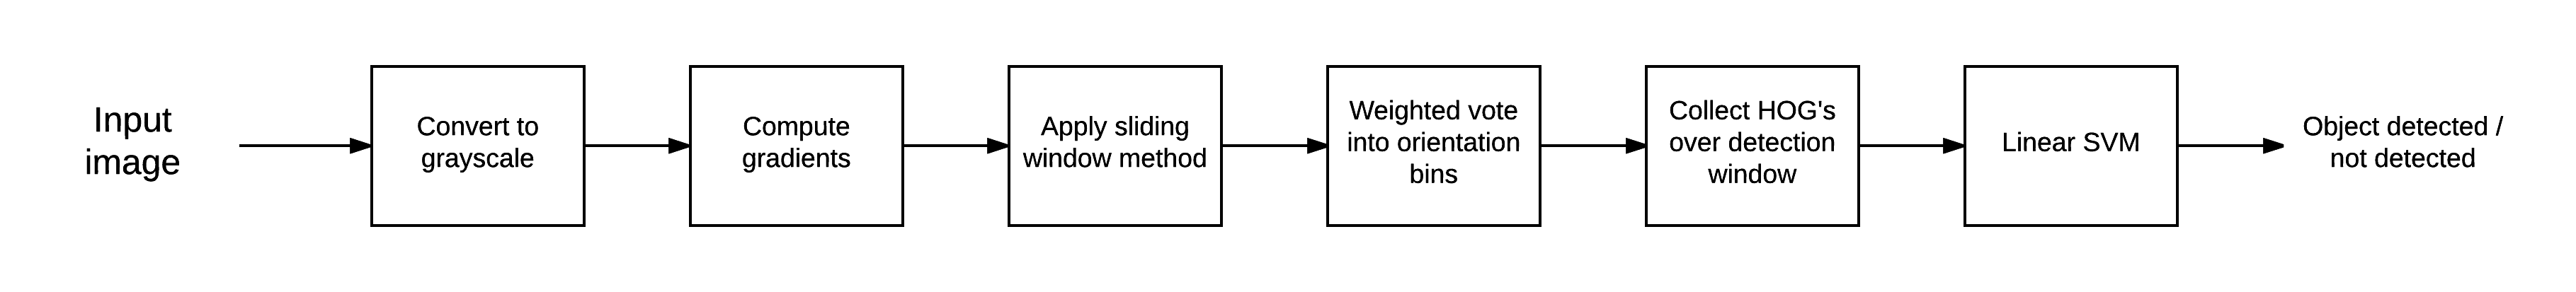
\includegraphics[width=15cm]{Process_of_detecting_an_object_with_HOG}
	\end{center}
	\caption[Process flow of detecting an object in an image]{The step-by-step process of detecting an object in an image generalized from the person detection method presented in \cite{DalalTriggs05}}
\end{figure}
The process of computing the HOG descriptor for a window as described in \cite{DalalTriggs05} respects the following steps: 
Firstly, the image is converted from RGB space to grayscale applying for each pixel the following formula: $0.2989 * R + 0.5870 * G + 0.1140 * B$, where R, G and B are the values of the red, green, respectively blue channel of the RGB image.	This way we're normalizing the colours. 
Secondly, a detection window of size $64\times128$ is used to slide over the gray image with a step of 32 pixels.
Then for each position, the window is divided in four $16\times16$ pixel blocks of four $8\times8$ pixel cells.
For each pixel cell, a histogram of 9 orientation bins in $0^{\degree}-180{\degree}$ (unsigned gradient) range is computed from the gradients of each pixel. This can be seen as a voting scheme, where each pixel contributes to a single orientation bin. As presented in \cite{DalalTriggs05} increasing the number of bins beyond 9 brings little accuracy improvement and allowing signed orientation bins in the range $0^{\degree}-360^{\degree}$ decreases the performance.
The gradient orientation for each pixel is computed as being $tan^{-1}\frac{g_{y}}{g_{x}}$ where $g_{x}$ and $g_{y}$ are the gradients with respect to the $x\ axis$, respectively $y\ axis$, calculated with the one of the several discrete derivative masks as 1-D point derivative (uncentred 
$
(
\begin{smallmatrix}
	-1 & +1
\end{smallmatrix}), 
$
centred 
$(
\begin{smallmatrix}
-1 & 0 & +1
\end{smallmatrix}),
$cubic corrected
$
 ( 
\begin{smallmatrix}
	-1 & -8 & 0 & +8 & +1
\end{smallmatrix})
$)
, $3\times3$ Sobel mask
$
\bigl(
\begin{smallmatrix}
	+1 & 0 & -1 \\
	+2 & 0 & -2 \\
	+1 & 0 & -1 \\
\end{smallmatrix}
\bigr)
$ or 2-D diagonal ones 
$
(
\begin{smallmatrix}
	 0 & 1\\
    -1 & 0
\end{smallmatrix}
),
(
\begin{smallmatrix}
	-1 & 0\\
	 0 & -1
\end{smallmatrix}
)
$. As concluded in \cite{DalalTriggs05} simple, 1-dimensional $(\begin{smallmatrix}
-1 & 0 & 1
\end{smallmatrix})$ masks work best. The histograms computed for each $8\times8$ pixel cells are concatenated resulting in a vector of 36 features. Lastly, for the entire window containing four $16\times16$ pixel blocks results, by concatenation, a feature vector of 144 dimensions.
This descriptor is then used to determine whether in the current window appears an instance of an object that we are looking for.
